\documentclass[11pt,a4paper]{article}
\usepackage[margin=2.3cm]{geometry}
\usepackage{graphicx}
\usepackage{booktabs}
\usepackage{xcolor}
\usepackage[colorlinks=true,linkcolor=blue!55!black,urlcolor=blue!55!black]{hyperref}
\usepackage{caption}
\captionsetup{font=small,labelfont=bf}
\graphicspath{{results/}}
\setlength{\parskip}{0.5em}
\setlength{\parindent}{0pt}

\title{\textbf{Section 2, Question 2}\\[0.3em]
       \large Real-Time Log Analytics with gRPC}
\author{Distributed Systems --- Homework 3}
\date{}

\begin{document}
\maketitle
\vspace{-2.5em}

\section{What the question asks}

Question~1 computed the Homework~2 Question~7 statistics over a file, as a batch
job that reads everything and then finishes. This question asks for the same
statistics over a \textbf{live stream}: records arrive continuously, and the
answers must be available \emph{while data is still arriving}.

The system must be distributed over several machines and built on gRPC, with
four participants --- a stream client that sends records, a coordinator that
receives and distributes them, workers that count, and query clients that ask
for the analytics at any moment. The final answer must still equal the
sequential program's, byte for byte.

\section{Architecture}

\begin{center}\small
\begin{tabular}{@{}lll@{}}
\toprule
\textbf{RPC} & \textbf{gRPC shape} & \textbf{Purpose} \\
\midrule
\texttt{StreamRecords} & client-streaming & the entire log stream, as one call \\
\texttt{GetAnalytics} & unary & one question, one answer \\
\texttt{WatchAnalytics} & server-streaming & the dashboard is pushed updates \\
\texttt{Worker.Process} & client-streaming (internal) & coordinator $\rightarrow$ worker \\
\texttt{Worker.GetStats} & unary (internal) & coordinator asks for totals \\
\bottomrule
\end{tabular}
\end{center}

All four gRPC call shapes are used, each where it genuinely fits rather than for
the sake of coverage. On the cluster the processes are placed one per machine:
the coordinator on the first, the clients on the second, one worker on each
remaining machine, so nothing shares a CPU.

\subsection{Design decisions, and why}

\textbf{The whole stream is one RPC.} \texttt{StreamRecords} is a single
client-streaming call rather than one call per batch, so the cost of
establishing a call is paid once. gRPC's own flow control then provides
backpressure without any code: if the coordinator cannot keep up, sending simply
slows down at the client.

\textbf{Records travel in columnar batches.} A \texttt{RecordBatch} holds one
list per field --- all the timestamps, then all the server identifiers --- rather
than a list of record objects. Protobuf encodes a list of integers far more
compactly than the same integers scattered across many small messages. This
turns out to be the single largest performance lever in the system.

\textbf{Workers send totals, not deltas.} A worker always reports its full
running totals, and the coordinator \emph{replaces} that worker's contribution
rather than adding to it. This makes asking safe to repeat: if a reply is lost,
the coordinator simply asks again, and nothing is counted twice. An earlier
design used epoch-numbered deltas with acknowledgements; it was the hardest part
of the system to explain, and removing it lost nothing.

\textbf{Bounded queues.} Each worker has a fixed-size queue. When a worker falls
behind, its queue fills, the coordinator blocks, and that blocking propagates
back through gRPC to the client. Memory stays bounded rather than growing until
the process dies.

\textbf{Mergeability and integer time.} As in Question~1, every figure is a
count, sum, minimum or maximum, so partial results combine in any order.
Averages are never stored --- a sum and a count are, and the division happens at
printing time. Response times are whole numbers of millionths of a millisecond,
so no ordering of workers can change the final digit.

\section{Results}

One million records, four workers unless stated, median of three runs, every run
checked against the sequential program.

\subsection{Workers}

\begin{center}\small
\begin{tabular}{@{}rrr@{}}
\toprule
\textbf{Workers} & \textbf{Throughput} & \textbf{Speedup} \\
\midrule
1 & \phantom{0,}823{,}037 rec/s & $1.00\times$ \\
2 & 1{,}573{,}037 rec/s & $1.91\times$ \\
4 & 2{,}909{,}799 rec/s & $\mathbf{3.54\times}$ \\
\bottomrule
\end{tabular}
\end{center}

Scaling is close to linear because workers never communicate with one another:
each holds its own totals and is merged only when someone asks. The shortfall
from $4\times$ is the coordinator, which parses and routes every record itself
and is therefore the one part that cannot be divided.

\subsection{Message granularity --- the dominant factor}

\begin{center}\small
\begin{tabular}{@{}rrr@{}}
\toprule
\textbf{Records per message} & \textbf{Throughput} & \textbf{vs one at a time} \\
\midrule
\phantom{00,}1 & \phantom{0,00}10{,}211 rec/s & $1\times$ \\
\phantom{0,0}10 & \phantom{0,0}99{,}199 rec/s & $10\times$ \\
\phantom{0,}100 & \phantom{0,}832{,}628 rec/s & $82\times$ \\
1{,}000 & 2{,}909{,}799 rec/s & $\mathbf{285\times}$ \\
10{,}000 & 3{,}124{,}137 rec/s & $306\times$ \\
\bottomrule
\end{tabular}
\end{center}

This spans more than two orders of magnitude and dwarfs every other variable
measured. Each message carries a fixed cost --- a protobuf header, a length
prefix, a pass through gRPC's machinery, a queue operation --- and at one record
per message that fixed cost \emph{is} the workload. The curve flattens beyond a
thousand records per message, where the fixed cost has become negligible
relative to the payload, so a thousand is the default.

The practical lesson generalises beyond this system: when an RPC framework seems
slow, the first thing to examine is how much work each call carries, not the
framework.

\subsection{Routing strategy}

\begin{center}\small
\begin{tabular}{@{}lrl@{}}
\toprule
\textbf{Strategy} & \textbf{Throughput} & \textbf{How it chooses} \\
\midrule
\texttt{round\_robin} & 2{,}909{,}799 rec/s & next worker in turn \\
\texttt{least\_loaded} & 1{,}822{,}886 rec/s & the worker with the shortest queue \\
\texttt{hash\_server} & \phantom{0,}221{,}908 rec/s & by server identifier \\
\bottomrule
\end{tabular}
\end{center}

\textbf{Even splitting beats clever splitting}, and by a wide margin.
\texttt{hash\_server} sends every record for a given server to the same worker;
the dataset contains a handful of busy servers, so one worker receives most of
the traffic while the others idle --- $13\times$ slower. \texttt{least\_loaded}
inspects queue depths on every batch, and that inspection costs more than the
imbalance it avoids.

Since the analytics are mergeable, there is no correctness reason to keep a
server's records together, so the simplest possible policy is also the fastest.

\subsection{The cost of querying during ingestion}

\begin{center}\small
\begin{tabular}{@{}rrr@{}}
\toprule
\textbf{Query clients} & \textbf{Ingest throughput} & \textbf{Query p99} \\
\midrule
\phantom{0}0 & 2{,}909{,}799 rec/s & --- \\
\phantom{0}1 & 2{,}388{,}961 rec/s & \phantom{0}32\,ms \\
\phantom{0}4 & \phantom{0,}779{,}990 rec/s & \phantom{0}42\,ms \\
16 & \phantom{0,}197{,}263 rec/s & 192\,ms \\
\bottomrule
\end{tabular}
\end{center}

Queries \emph{are} served while data streams in, which is what the question
asks for --- but they are not free. Sixteen closed-loop query clients cost
$15\times$ the ingestion rate. Each query makes the coordinator collect and
merge every worker's totals, and that work competes directly with routing
records.

This is precisely why \texttt{WatchAnalytics} exists. A dashboard subscribed to
the server stream is \emph{pushed} updates from one periodic merge, so ten
observers cost one round of work rather than ten. Polling with
\texttt{GetAnalytics} is the expensive pattern; subscribing is the cheap one.

\begin{figure}[htbp]
\centering
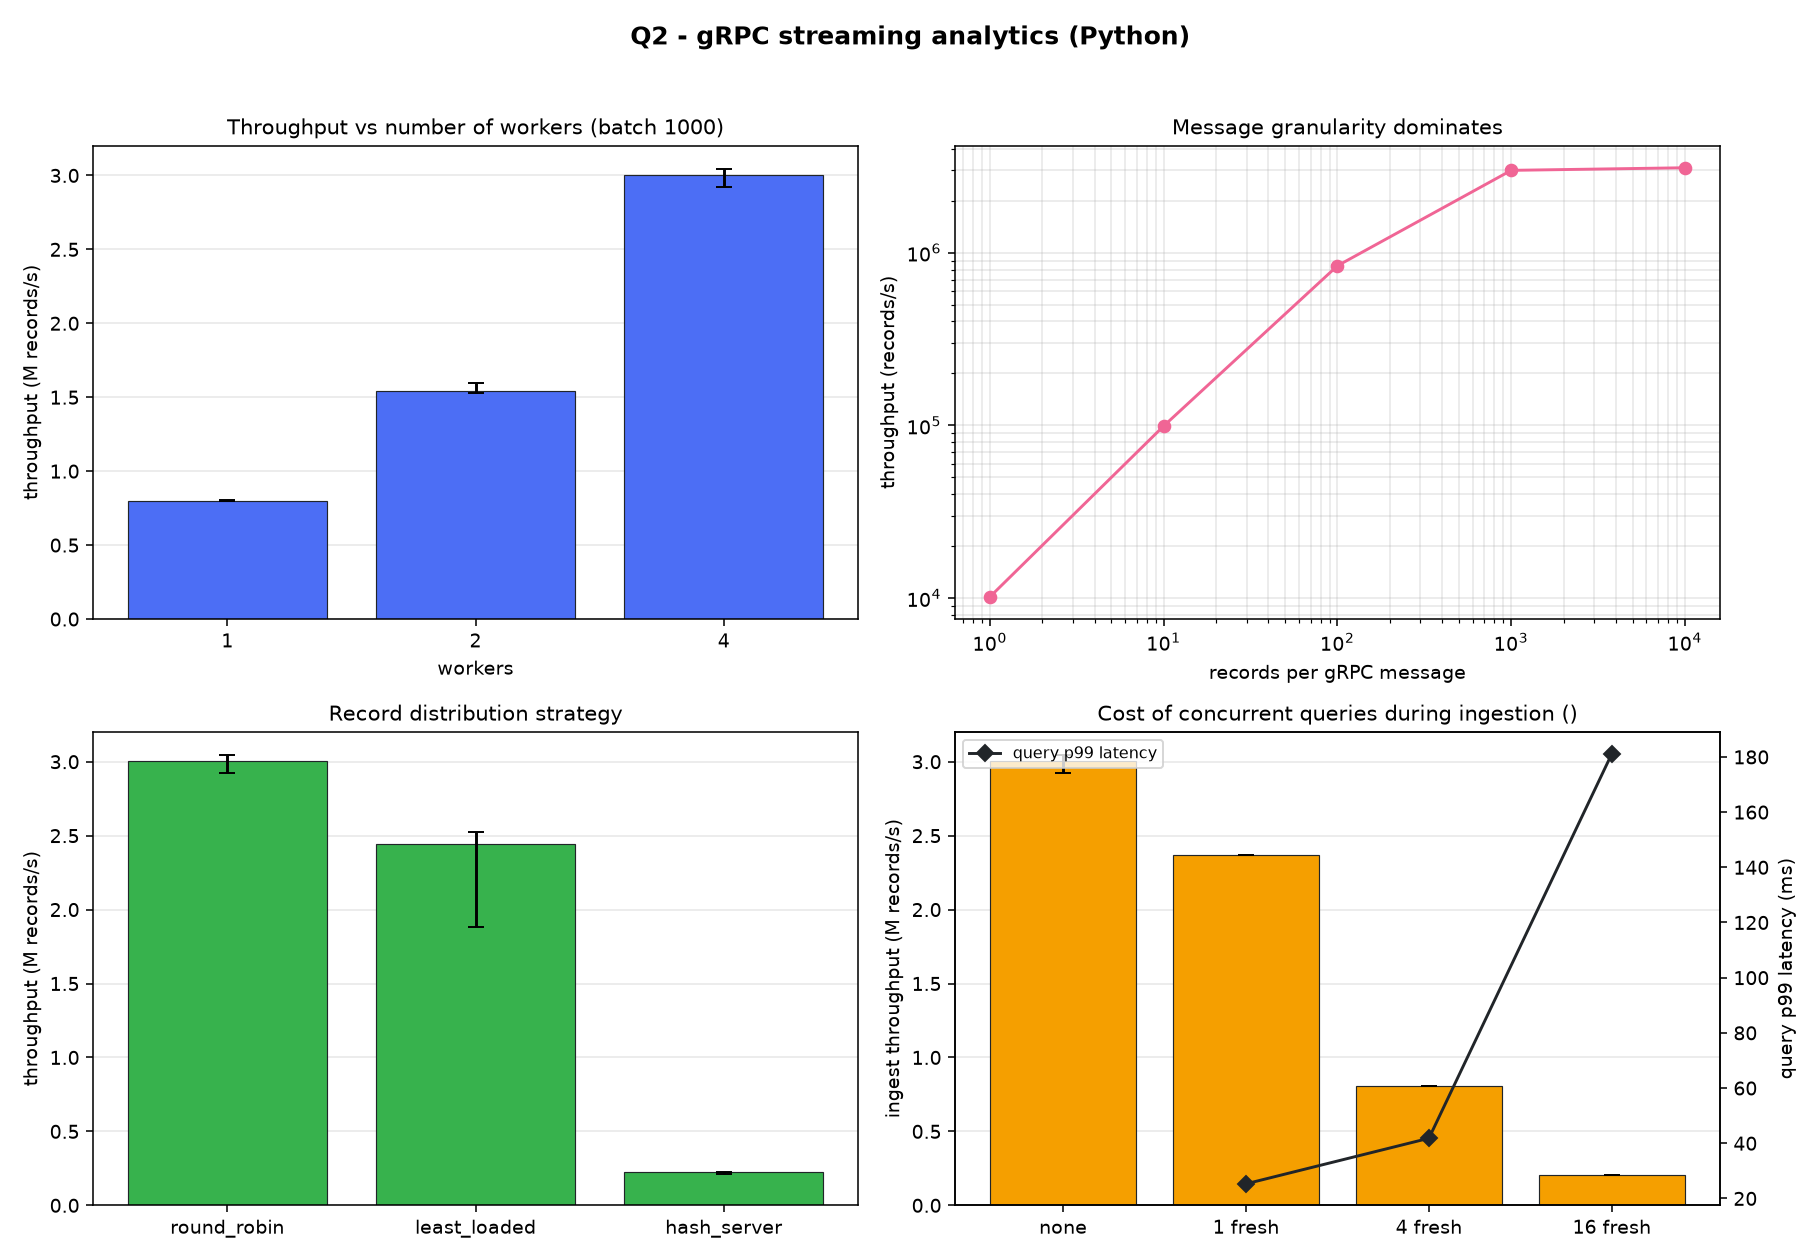
\includegraphics[width=\textwidth]{q2_plots.png}
\caption{The four sweeps: throughput against worker count; the effect of message
granularity, spanning two orders of magnitude; the comparison of routing
strategies; and the cost of concurrent queries during ingestion, with query
latency on the right-hand axis.}
\end{figure}

\begin{figure}[htbp]
\centering
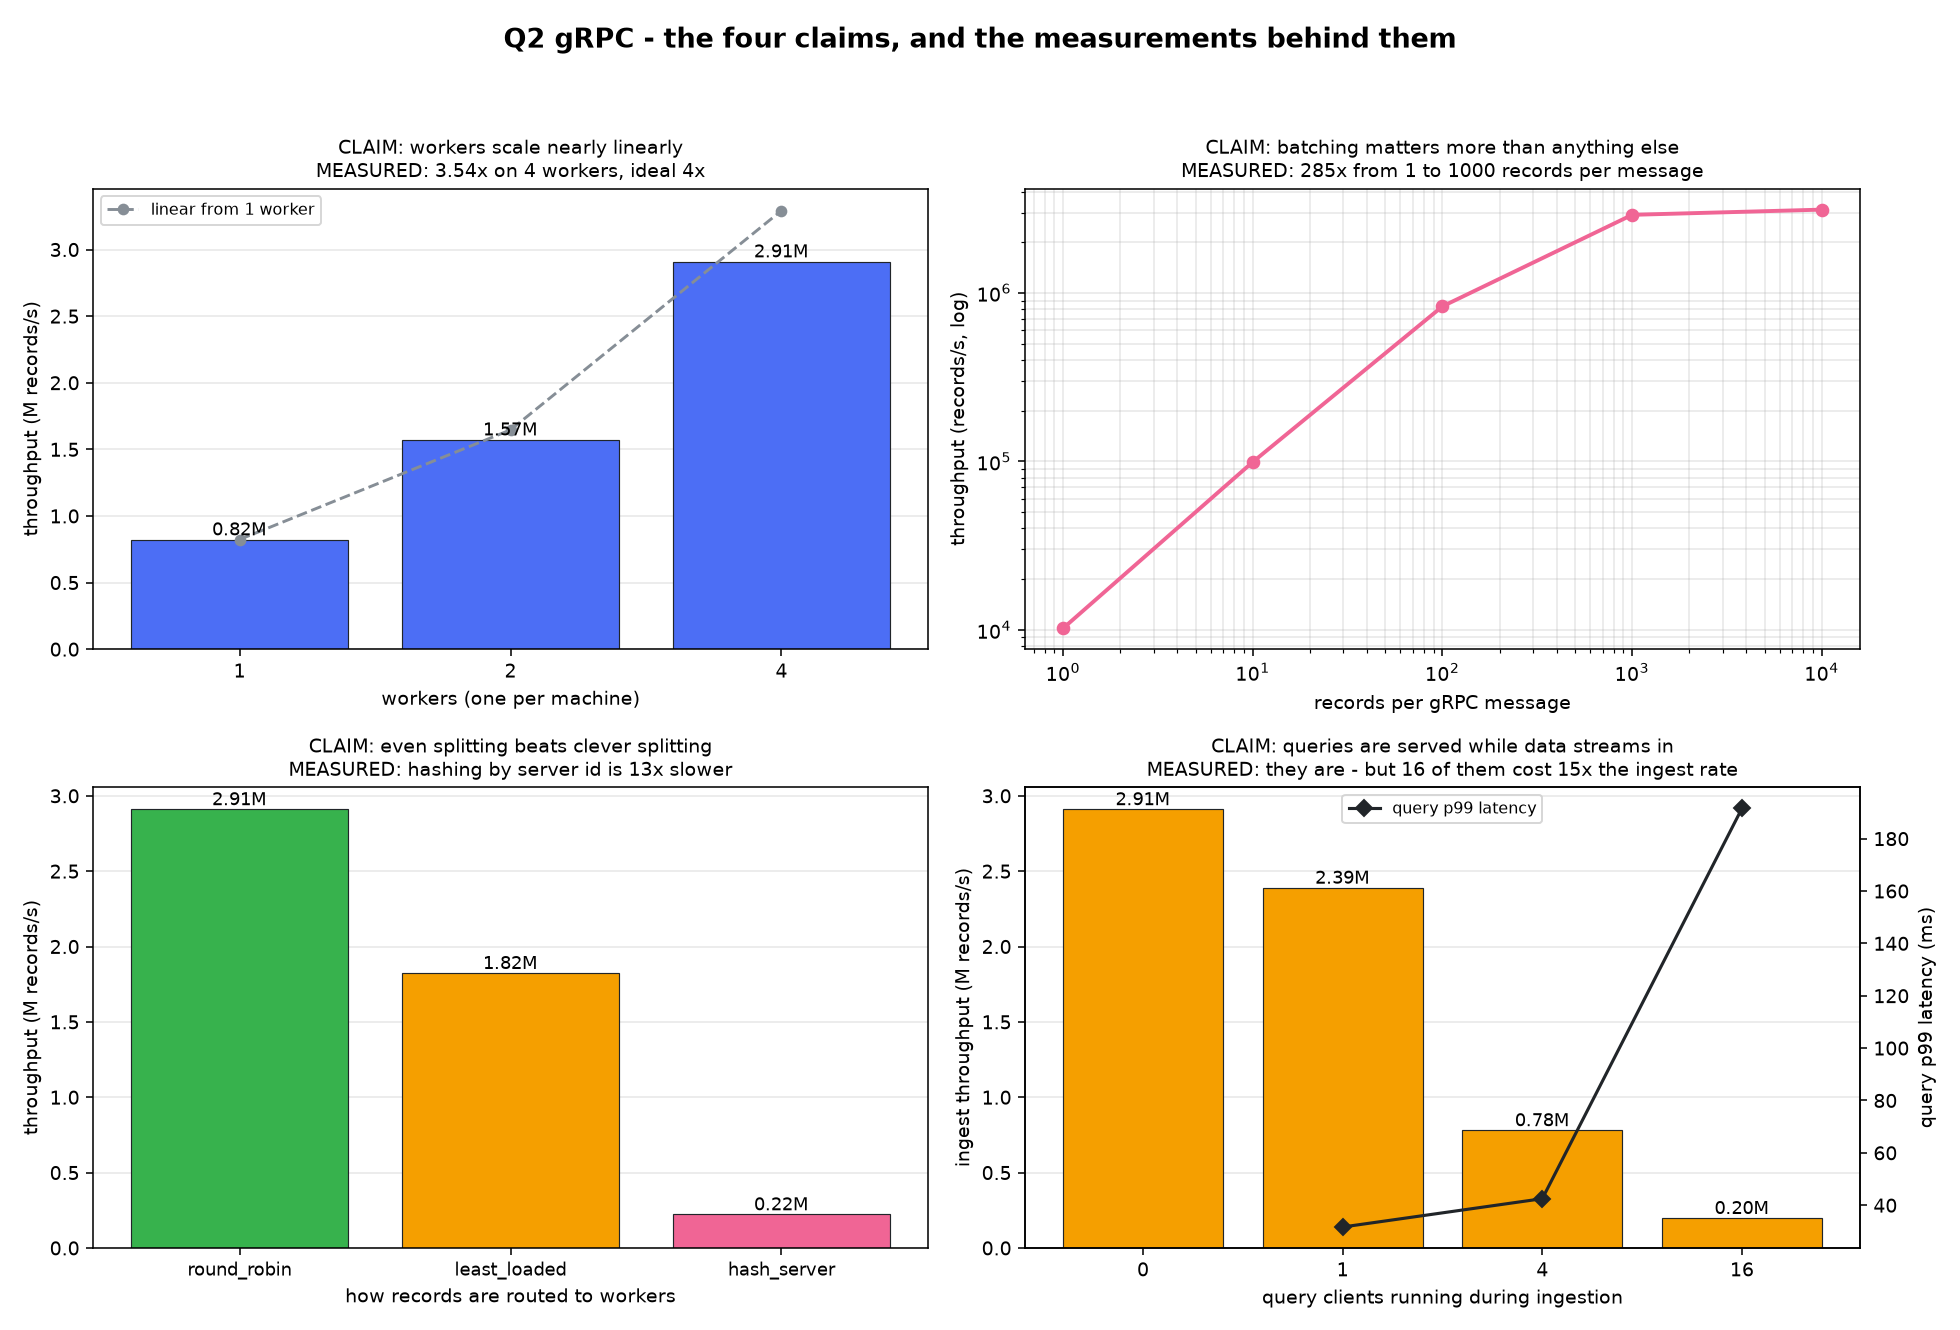
\includegraphics[width=\textwidth]{q2_facts.png}
\caption{Each claim made about the system, set beside the measurement that
supports it. Stating a claim and its evidence together is what distinguishes a
design that was measured from one that was merely asserted.}
\end{figure}

\section{Comparison with the batch implementations}

All three implementations compute the same analytics over the same
one-million-record file on four machines.

\begin{center}\small
\begin{tabular}{@{}lrr@{}}
\toprule
\textbf{Implementation} & \textbf{Throughput} & \textbf{Time for 1M records} \\
\midrule
MapReduce (Question 1) & 1.35M rec/s & 0.74\,s \\
MPI (Homework 2 baseline) & 2.09M rec/s & 0.48\,s \\
gRPC streaming (this work) & \textbf{2.91M rec/s} & \textbf{0.34\,s} \\
\bottomrule
\end{tabular}
\end{center}

This ordering is \textbf{not} a ranking of the three technologies, and it would
be dishonest to present it as one. MapReduce and MPI read the file from disk and
terminate; this system receives records over the network and continues answering
queries throughout, and its figure excludes reading a file because a real stream
has no file to read.

What the comparison does establish is worth stating plainly: the streaming
design pays \textbf{no penalty for being incremental}. Maintaining a queryable
answer at every instant --- rather than producing one answer at the end --- costs
nothing in throughput here. The batch systems have no advantage to give up.

\begin{figure}[htbp]
\centering
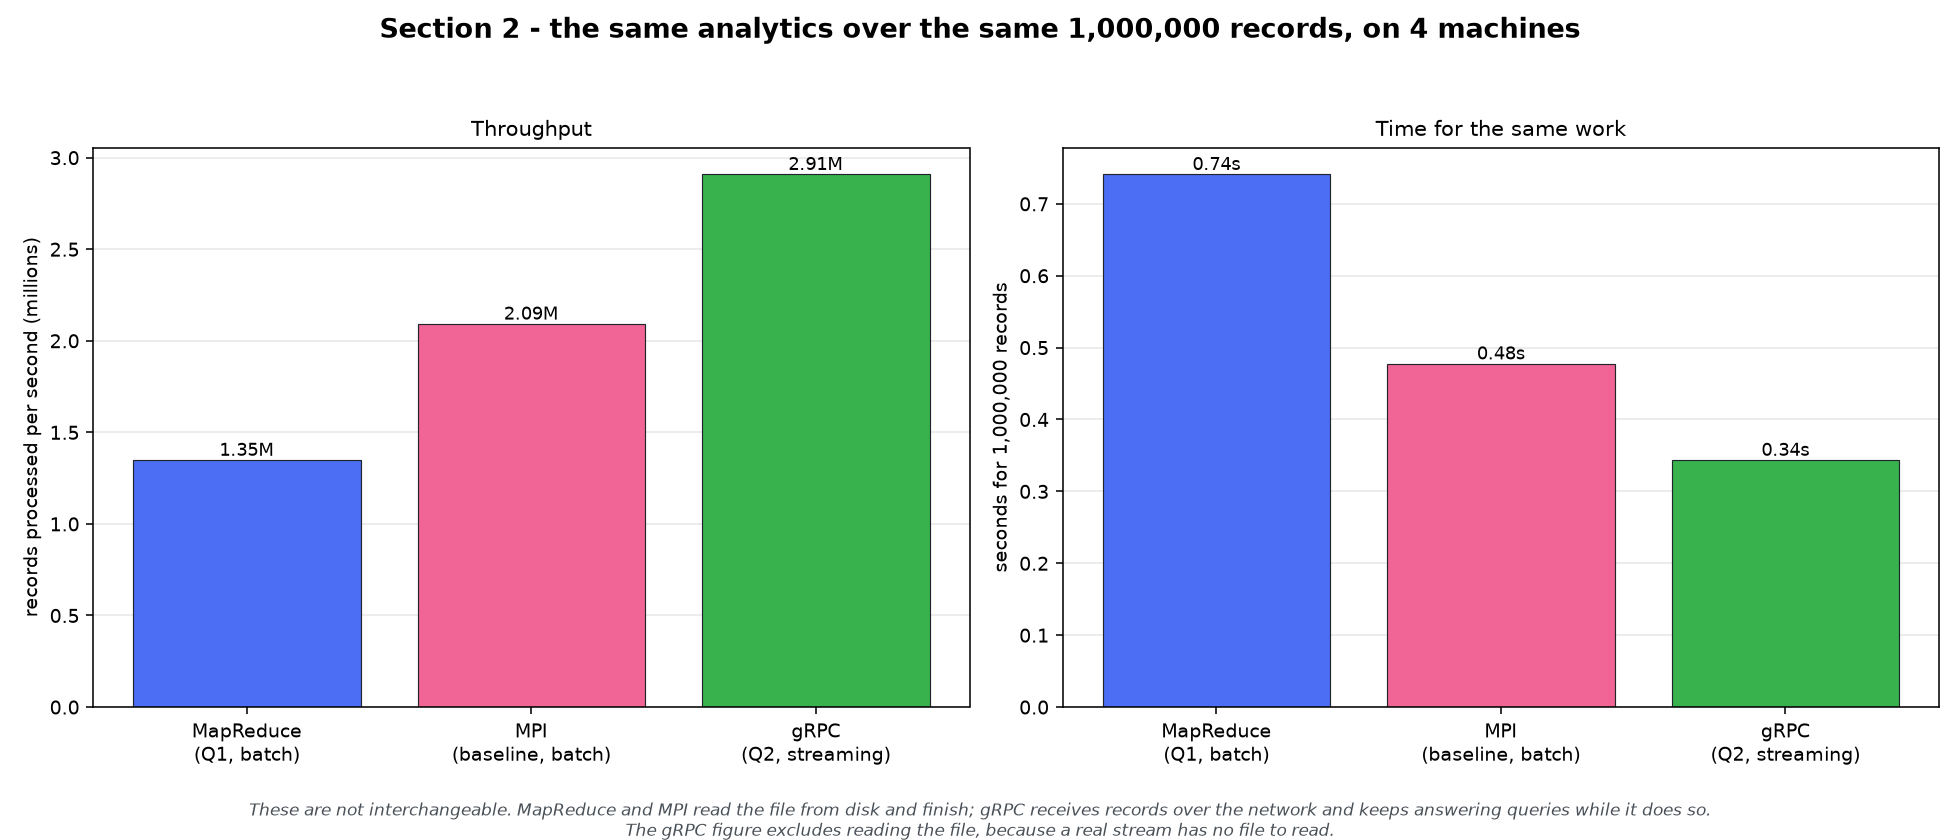
\includegraphics[width=\textwidth]{paradigm_compare.png}
\caption{MapReduce, MPI and gRPC over identical work on four machines. The
caveat about what is and is not being compared is printed on the figure itself,
so it cannot become separated from the numbers.}
\end{figure}

\section{Correctness}

Seventy-six checks, all passing. They sweep worker counts, all three routing
strategies, batch sizes from 1 to 10{,}000, several concurrent stream sources,
and queries issued mid-stream --- each time comparing the system's final answer
against Question~1's \texttt{log\_seq}, the unmodified Homework~2 sequential
program. Using one oracle for both questions rather than two means the two
implementations cannot quietly disagree with each other.

The checks that matter most are the ones where the answer could plausibly have
differed: several sources streaming at once, a query issued halfway through, and
a reset followed by a fresh stream. Distribution is only correct if the result
does not depend on timing, and those are the cases where timing varies.

\section{Conclusions}

The system sustains roughly $2.9$ million records per second on four machines
while answering queries concurrently, and its final answer is byte-identical to
the sequential program under every configuration tested.

Three findings are worth carrying forward. Message granularity dominates
everything else, by $285\times$ --- far more than worker count or routing policy.
The simplest routing policy is the fastest, because mergeable analytics impose
no requirement to keep related records together. And concurrent queries are
genuinely affordable only when observers subscribe rather than poll, which is
what the server-streaming RPC is for.
\end{document}
